\documentclass[a4paper,11pt]{article}
\usepackage{exptech}
\usepackage{textcomp}
\usepackage{graphicx}
\usepackage{array}
\usepackage[babel=true]{csquotes}
\usepackage{url}
\usepackage{hyperref}
\usepackage{wrapfig}
\usepackage[export]{adjustbox}
\usepackage{titletoc}
\usepackage{placeins}

\titlecontents{subsection}[3.8em]{}{}{}{}[\addvspace{-0.5pt}]
\hypersetup{
  bookmarks=true, % show bookmarks bar?
  pdftitle={Avalon - Rapport de spécifications fonctionnelles}, % title
  pdfnewwindow=true, % links in new window
  colorlinks=true, % false: boxed links; true: colored links
  linkcolor=black, % color of internal links (change box color with linkbordercolor)
  citecolor=cyan, % color of links to bibliography
  filecolor=cyan, % color of file links
  urlcolor=cyan % color of external links
}

\title{
  \textbf{Avalon}\newline
  Rapport de spécifications fonctionnelles
}
\markright{Avalon - Rapport de spécifications fonctionnelles}
\author{
\begin{minipage}{0.4\textwidth}
	\begin{flushleft} \large
		\emph{Auteurs :}\\
		Alexandre \textsc{Audinot}\\
		Julien \textsc{Bouvet}\\
		Cyrille \textsc{Delabre}\\
		Thierry \textsc{Gaugry}\\
		Nicolas \textsc{Hurman}\\
		Léo \textsc{Jacoboni}\\
		Alexandre \textsc{Leonardi}\\
	\end{flushleft}
\end{minipage}
\begin{minipage}{0.4\textwidth}
	\begin{flushright} \large
		\emph{Encadrants :} \\
		Valérie \textsc{Gouranton}\\
		Ronan \textsc{Gaugne}\\
		Bruno \textsc{Arnaldi}\\
		Willy \textsc{Allègre}\\
		Jean-Paul  \textsc{Departe}\\
	\end{flushright}
\end{minipage}
}


\date{27 novembre 2014}

\begin{document}
\maketitle
\thispagestyle{empty}

\begin{figure}[h!]
   \begin{minipage}{0.3\linewidth}
      
\includegraphics[scale=0.9]{2-Specifications/img/logo_insa.jpeg}
   \end{minipage}
   \begin{minipage}{0.2\linewidth}
      \centering
      
\includegraphics[scale=0.5,left]{2-Specifications/img/logo_irisa.jpg}
   \end{minipage}\hfill
   \begin{minipage}{0.2\linewidth}
      
\includegraphics[scale=0.9]{2-Specifications/img/logo_kerpape.png}
   \end{minipage}
\end{figure}


\pagebreak

\tableofcontents
\pagebreak


\section{Introduction}

% Annonce plan
% Visite kerpape
% Rencontre clients
\begin{wrapfigure}{r}{0mm}
	\centering
	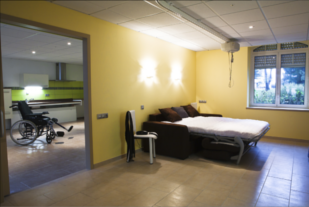
\includegraphics[scale=1]{1-PreEtude/img/appt_tremplin_intro.png}
\end{wrapfigure}
Notre projet consiste en la modélisation d'appartements tremplins en 3D pleinement interactifs, dans lesquels des personnes handicapées pourront évoluer et apprendre à se servir des différents équipements de domotique présents. 
Le projet est proposé par le centre de rééducation de Kerpape et par l'IRISA, ce qui lui confère un intérêt particulier à nos yeux car le commanditaire est extérieur à l'école, et le projet répond donc au besoin d'un véritable client de la même manière que le ferait un projet rencontré dans notre vie professionnelle. 
Ainsi, nous avons eu l'occasion de nous entretenir avec Willy Allègre et Jean-Paul Departe, ingénieurs de Kerpape à l'origine du projet, tout d'abord lors d'une conférence téléphonique pendant laquelle ils nous ont décrit ce qu'ils attendaient de l'application. Par la suite, un déplacement au centre de Kerpape nous a permis de parfaire l'image que nous nous faisons du résultat attendu et de compléter le cahier des charges de la future application. \newline

\begin{wrapfigure}{l}{0mm}
	%\cite{archeologie}
	\centering
	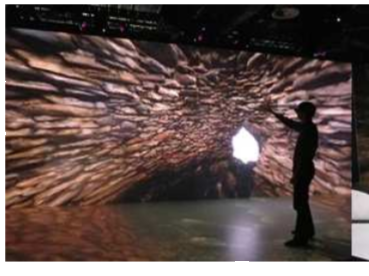
\includegraphics[scale=0.5]{1-PreEtude/img/rv_2.png}
\end{wrapfigure}
Au cours de cette étude de pré-spécifications, nous commencerons par définir plus précisément le contexte de notre projet, en tentant de cerner ce qu'est la réalité virtuelle et son importance dans le domaine de la santé. 
Nous présenterons ensuite le cahier des charges en deux parties, d'abord d'un point de vue fonctionnel, les différentes fonctions qui sont attendues de notre applications, et ensuite d'un point de vue technique, les différentes contraintes que nous aurons à respecter. 
Après cela nous décrirons, dans l'étude fonctionnelle, les différents scénarios types qui nous ont été proposés par Kerpape et auxquels les patients devront pouvoir être confrontés. 
Puis nous spécifierons les différents logiciels à notre disposition ainsi que les différents matériels, et les périphériques que nous prévoyons de rendre utilisables. 
Enfin, nous ébaucherons une planification prévisionnelle du travail à fournir tout au long de l'année. 
\pagebreak
\section{Environnement logiciel et matériel}

Dans notre rapport précédent, nous définissions un cahier des charges qui s'articulait principalement autour de 3 grands axes qui étaient les suivants : 
\begin{itemize}\renewcommand{\labelitemi}{$\bullet$}
\item Présence d'interactions avec l'environnement
\item Applications aisément portable vers différents systèmes d'utilisation
\item Exploitation de différents périphériques d'entrée/sortie
\end{itemize}
Nous allons donc dans un premier temps présenter les solutions techniques que nous avons retenues pour la réalisation du projet, en détaillant de quelle façon elles répondent à ces 3 problématiques, pour ensuite énumérer les différents scénarios d'utilisation que nous allons implémenter, avant d'enfin détailler les différentes cibles de déploiement prévues. 

\subsection{Solutions techniques retenues}
La réalisation de notre projet s'appuiera principalement sur trois environnements de travail, Unity3D, Blender et MiddleVR.

\subsubsection{Unity : le moteur de rendu 3D}
L'utilisation d'Unity était imposée, en vertu des nombreux avantages du logiciel. Unity (fig. \ref{screen_unity}) est un moteur de rendu 3D
\begin{wrapfigure}{l}{0mm}
	\centering
	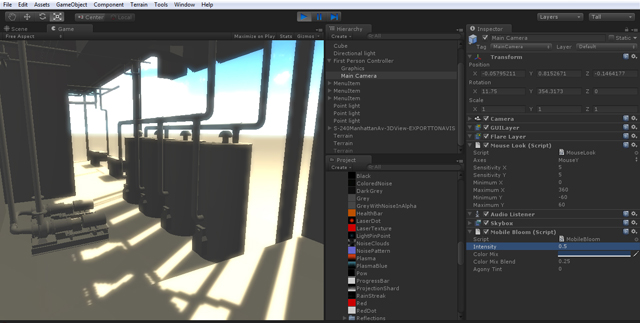
\includegraphics[scale=0.5]{2-Specifications/img-utilisateur/screen_unity.jpg}
	\caption{Capture d'écran Unity3D}
	\label{screen_unity}
\end{wrapfigure}
utilisé principalement pour la réalisation de jeux vidéos, et qui dispose d'une version gratuite. Très complet, il propose les différentes fonctionnalités dont nous avons besoin : il permet d'ouvrir le modèle 3D de l'appartement tremplin qui nous a été fourni par le centre de Kerpape, et de le modifier. \newline

Il permet aussi de réaliser les interactions entre utilisateur et environnement qui nous intéressent, que ce soit l'appui sur les différents interrupteurs gérant l'éclairage et l'ouverture/fermeture des volets, ou bien l'utilisation de la télécommande dont disposent les résidents de l'appartement qui centralise la plupart des actions qu'ils peuvent effectuer.
Enfin dernier avantage de Unity, il propose différentes cibles de compilation. En effet, même si dans un premier temps nous allons développer une application qui fonctionnera sous Windows 7 ou 8 avec un ensemble clavier/souris, nous aimerions ne pas être limités à cet environnement par la suite. \newline

Néanmoins, un problème est survenu lors de l'utilisation de Unity : le modèle 3D de l'appartement qui nous a été fourni avait été créé grâce à 3DSMax, et les deux logiciels sont réputés incompatibles entre eux, ce qui s'est avéré dans notre cas. Nous avons donc au final obtenu un modèle contenant les volumes, mais sans texture ni lumière, que nous avons dû ajouter nous-mêmes. 

\subsubsection{Blender : le logiciel de modélisation}
Blender est le logiciel de modélisation que nous allons utiliser pour les modifications du modèle qui nous a été fourni. Contrairement à Unity, il ne nous a pas été imposé, mais s'est dégagé comme étant le choix idéal du fait de la documentation imposante disponible sur le net et de sa gratuité.\newline
La majorité de l'appartement tremplin a déjà été modélisé pour nous, mais il reste néanmoins quelques détails à rajouter, comme l'interphone/téléphone (le domophone), ou encore le panneau d'interrupteurs à l'entrée de l'appartement. Nous nous en servirons de plus pour corriger les pertes rencontrées lors de l'import du modèle 3D sous Unity : rajouter la lumière et les textures à notre modèle. 

\subsubsection{MiddleVR : la gestion des périphériques d'interaction}

MiddleVR répond au troisième des objectifs que nous nous sommes fixés : exploiter différents périphériques d'entrée/sortie. En effet, pour ce faire, il fallait pouvoir s'abstraire desdits périphériques au cours du développement de l'application. L'idée est de développer toutes les fonctionnalités qui nous intéressent, l'utilisation des différents interrupteurs, etc, et d'ensuite disposer d'un moyen facile d'associer l'usage d'un périphérique donné à une fonctionnalité donnée.\newline
Or c'est précisément ce que nous permet MiddleVR. Il est capable de reconnaître les différents périphériques de réalité virtuelle à notre disposition, pour ensuite les associer à certaines parties du corps comme la tête ou la main. Cela nous permet, lors de l'utilisation de Unity, de réaliser des interactions qui ne vont pas se  baser sur une wiimote ou une souris, mais sur la main de l'utilisateur, quel que soit le périphérique que MiddleVR lui a associé. 

\subsection{Déploiement}
Parmi nos 3 axes de développement, l'un était l'exploitation de différents périphériques d'entrée/sortie. Il y a, en pratique, 3 périphériques de sortie que nous prévoyons d'utiliser au cours du projet : un écran de PC classique, un casque de réalité virtuel type Occulus Rift, et la salle immersive Immersia de l'IRISA.

\subsubsection{Ecran}
Il s'agit de la première version que nous allons développer. Cette version pourra reconnaître différents périphériques d'entrée, mais sera au départ prévue pour des interactions \textit{via} le couple clavier/souris. Grâce à MiddleVR, cette option n'est pas plus ou moins facile à implémenter que les autres, mais elle représente un bon point de départ car elle ne nécessite pas d'équipement particulier, le centre de Kerpape disposant déjà de machines qui pourront faire tourner le programme. \newline

De  plus, bien que cette approche soit moins \enquote{naturelle} que l'usage de dispositifs de réalité virtuelle comme ceux associés à la salle Immersia, elle est au final aisée de prise en main car il s'agit de matériel auquel la plupart des gens sont déjà habitués.

\subsubsection{Casque de RV}
La première approche présentée, bien qu'étant la plus facile d'implantation, n'implique pas suffisament la notion de réalité virtuelle, actuellement à l'étude par le centre de Kerpape, qui souhaiterait savoir si la réalité virtuelle est adaptée à la préparation de ses patients à l’utilisation des appartements tremplins. 
En effet, un dispositif comme un casque de réalité virtuelle permet une meilleure immersion de l'utilisateur et permet de mieux gérer les différents types de handicaps : moins d'infrastructure à mettre en place, le patient n'a pas à se déplacer car l'ergothérapeute vient à lui, pas de risque de se blesser...
Et bien sûr la possibilité d'avoir plusieurs patients qui apprennent en même temps, chose impossible à l'heure actuelle (car un seul appartement est libre à la fois. 

Qui plus est, elle se marie avantageusement avec l'usage de dispositifs comme des manettes pour Nintendo Wii ou des Razer Hydra qui sont eux-mêmes plus immersifs que le classique clavier/souris, car ils permettent de retranscrire les mouvements réels que l'utilisateur fera avec ses mains. \newline
\begin{wrapfigure}{r}{0mm}
  \centering
  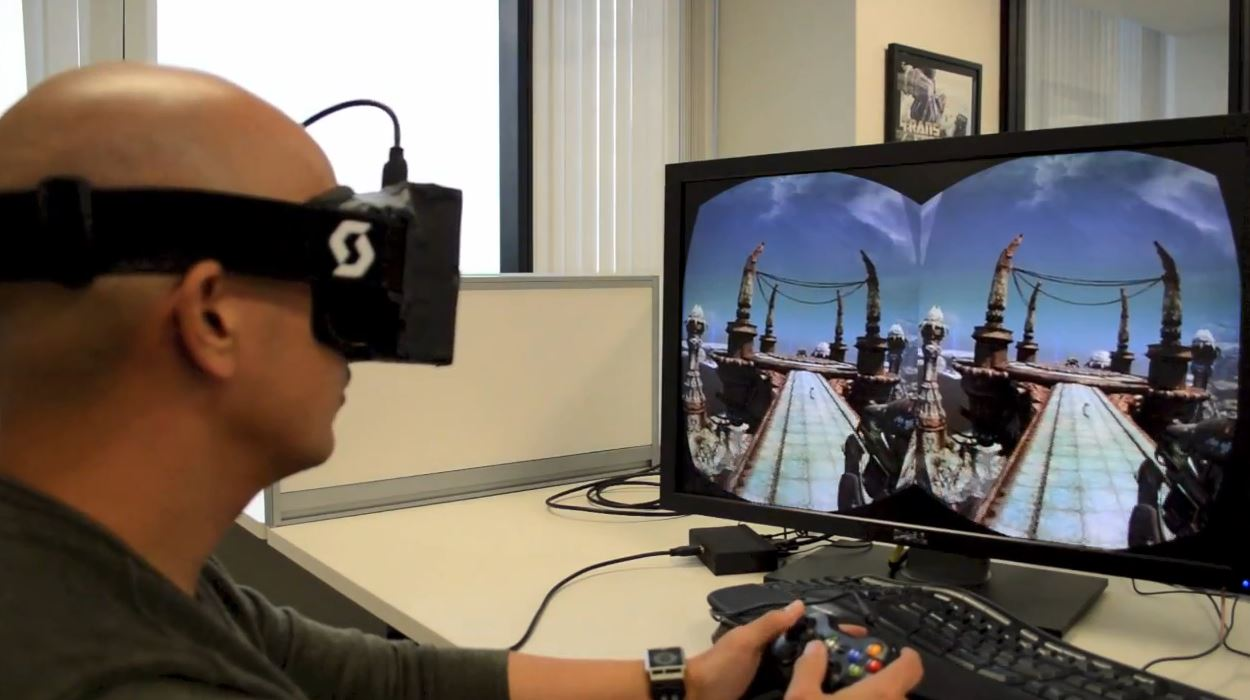
\includegraphics[scale=0.3]{2-Specifications/img-utilisateur/occulus.jpg}
	\caption{Casque de réalité virtuelle : Occulus Rift}
	\label{occulus_reparo}
\end{wrapfigure}
Lors de notre visite au centre de Kerpape nous avons fait essayer une démonstration de l'Occulus Rift (fig. \ref{occulus_reparo}) à Willy Allègre et Jean-Paul Departe, qui ont été plutôt convaincus de l'intérêt du dispositif. 
Les périphériques de ce type étant en pleine démocratisation, ils sont donc particulièrement intéressant financièrement pour un centre tel que Kerpape, car ne représentant qu'une fraction infime du prix d'un nouvel appartement témoins.

\subsubsection{Salle immersive}
La salle immersive (fig. \ref{immersiaaaaaaaa}) représente l'équipement de RV le plus complet dont nous puissions profiter et est donc une perspective de plate-forme très intéressante pour notre application.
%\begin{wrapfigure}{l}{0mm}
	%\centering
	%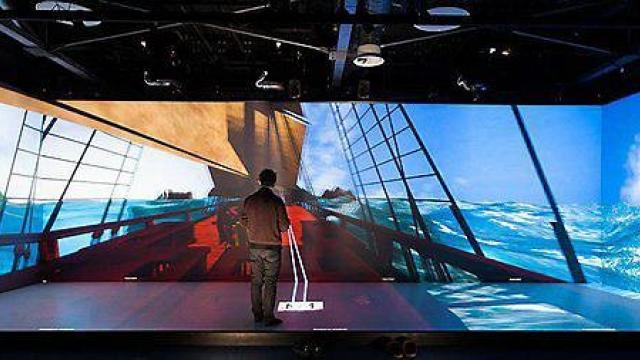
\includegraphics[scale=0.5]{2-Specifications/img-utilisateur/immersia.jpg}
	%\caption{Salle Immersia : plus grande salle de RV du monde}
	%\label{immersiaaaaaaaa}
%\end{wrapfigure}
C'est l'option qui nous permettra les interactions les plus naturelles, car l'utilisateur se trouvera dans une projection à l'échelle 1:1 de l'appartement, équipé de lunettes 3D et de capteurs qui permettent de suivre la position des mains de l'utilisateur. \newline
L'utilisation d'une plateforme de ce type permet d'éviter les quelques risques liée à l'utilisation de périphériques portés par l'utilisateur : leur poids, gênant pour les patients à handicap moteur, ou la perte de repères de son propre corps (pas de vision de ses membres).
Bien que Kerpape n'en dipose pas et n'ait pas la possibilité d'en utiliser une, l'implémentation du projet Avalon dans une salle immersive reste un objectif que nous souhaitons réaliser, car cela représente une évolution logique du projet.
L'utilisation d'une salle de ce type permet de laisser le projet ouvert à d'autres utilisations dans le domaine de la rééducation fonctionnelle et de le valoriser grâce à la visibilité d'Immersia.

\pagebreak
\section{Spécifications fonctionnelles du projet}

Dans notre rapport précédent, nous définission un cahier des charges qui s'articulait principalement autour de 3 grands axes qui étaient les suivants :
\begin{itemize}\renewcommand{\labelitemi}{$\bullet$}
\item Présence d'interactions avec l'environnement
\item Applications aisément portable vers différents systèmes d'utilisation
\item Exploitation de différents périphériques d'entrée/sortie
\end{itemize}
Nous allons donc dans un premier temps présenter les solutions techniques que nous avons retenues pour la réalisation du projet, en détaillant de quelle façon elles répondent à ces 3 problématiques, pour ensuite présenter un diagramme de cas d'utilisation qui résumera le fonctionnement global de l'application.

\subsection{Solutions techniques retenues}
La réalisation de notre projet s'appuiera donc principalement sur trois environnements de travail, Unity3D, Blender et MiddleVR.

\subsubsection{Unity : le moteur de rendu 3D}
L'utilisation d'Unity était imposée, en vertu des nombreux avantages du logiciel. Unity est un moteur de rendu 3D
\begin{wrapfigure}{l}{0mm}
	\centering
	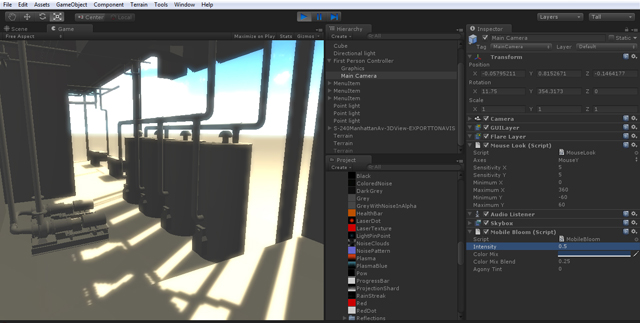
\includegraphics[scale=0.5]{2-Specifications/img-utilisateur/screen_unity.jpg}
\end{wrapfigure}
utilisé principalement pour la réalisation de jeux vidéos, et qui dispose d'une version gratuite. Très complet, il propose les différentes fonctionnalités dont nous avons besoin : il permet d'ouvrir le modèle 3D de l'appartement tremplin qui nous a été fourni par le centre de Kerpape, et de le modifier. \newline

Il permet aussi de réaliser les interactions entre utilisateur et environnement qui nous intéressent, que ce soit l'appui sur les différents interrupteurs gérant l'éclairage et l'ouverture/fermeture des volets, ou bien l'utilisation de la télécommande dont disposent les résidents de l'appartement qui centralise la plupart des actions qu'ils peuvent effectuer.
Enfin dernier avantage de Unity, il propose différentes cibles de compilation. En effet, même si dans un premier temps nous allons développer une application qui fonctionnera sous Windows 7 ou 8 avec un ensemble clavier/souris, nous aimerions ne pas être limités à cet environnement par la suite. \newline

Néanmoins, un problème est survenu lors de l'utilisation de Unity : le modèle 3D de l'appartement qui nous avait été fourni avait été créé grâce à 3DSMax, et les deux logiciels sont réputés incompatibles entre eux, ce qui s'est avéré dans notre cas. Nous avons donc au final obtenu un modèle contenant les volumes, mais sans texture ni lumière, que nous avons dû ajouter nous-mêmes.

\subsubsection{Blender : le logiciel de modélisation}
Blender est le logiciel de modélisation que nous allons utiliser pour les modifications du modèle qui nous a été fourni. Contrairement à Unity, il ne nous a pas été imposé, mais s'est dégagé comme étant le choix idéal du fait de la documentation imposante disponible sur le net et de sa gratuité.\newline

La majorité de l'appartement tremplin a déjà été modélisé pour nous, mais il reste néanmoins quelques détails à rajouter, comme l'interphone/téléphone (le domophone), ou encore le panneau d'interrupteurs à l'entrée de l'appartement. Nous nous en servirons de plus pour corriger les pertes rencontrées lors de l'import du modèle 3D sous Unity : rajouter la lumière et les textures à notre modèle.

\subsubsection{MiddleVR : la gestion des périphériques d'interaction}

MiddleVR répond au troisième des objectifs que nous nous sommes fixés : exploiter différents périphériques d'entrée/sortie. En effet, pour ce faire, il fallait pouvoir s'abstraire desdits périphériques au cours du développement de l'application. L'idée est de développer toutes les fonctionnalités qui nous intéressent, l'utilisation des différents interrupteurs, etc, et d'ensuite disposer d'un moyen facile d'associer l'usage d'un périphérique donné à une fonctionnalité donnée.\newline

Or c'est précisément ce que nous permet MiddleVR. Prenant la forme d'un plugin Unity disponible gratuitement, il est capable de reconnaître les différents périphériques de réalité virtuelle à notre disposition, pour ensuite les associer à certaines actions.

\subsection{Scénarios d'utilisation}
Le cahier des charges qui nous a été fourni par le centre de Kerpape prévoit l'implémentation de différents scénarios d'utilisation centrés sur l'usage du domophone et que nous avons détaillés dans le premier rapport :
\begin{itemize}\renewcommand{\labelitemi}{$\bullet$}
\item Appel téléphonique normal
\item Appel \textit{via} l'interphone d'une personne venant fréquemment (un infirmier par exemple)
\item Appel \textit{via} l'interphone concernant une visite inattendue
\end{itemize}
Ces scénarios mettent en avant l'usage particulier qui peut être fait du téléphone et de la télévision (cf. \textsc{figure~\ref{domophone}}), car ceux-ci servent d'interphone, respectivement pour le son et l'image. Il faut donc que le téléphone, dans notre application, puisse recevoir des appels des deux types différents, mais aussi que la TV puisse recevoir le flux vidéo de l'interphone (en pratique dans les appartements tremplins, l'habitant doit se placer sur le canal 80 pour afficher la caméra de l'interphone).
\begin{figure}[h!]
	\begin{center}
  		\caption{Cas d'utilisation du domophone}
  		\label{domophone}
  		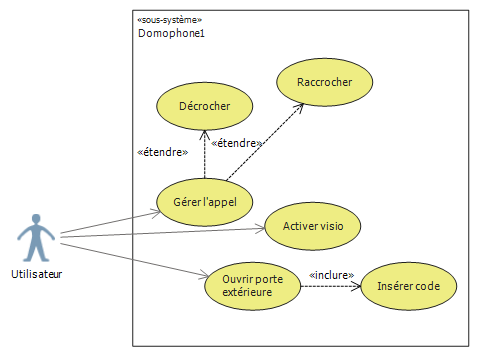
\includegraphics[width=\textwidth]{2-Specifications/img-utilisateur/use_case_diag.PNG}
  	\end{center}
\end{figure}

\subsection{Déploiement}
Parmi nos 3 axes de développement, l'un était l'exploitation de différents périphériques d'entrée/sortie. Il y a, en pratique, 3 périphériques de sortie que nous prévoyons d'utiliser au cours du projet : un écran de PC classique, un casque de réalité virtuel type Occulus Rift, et la salle immersive Immersia de l'IRISA.

\subsubsection{Ecran}
Il s'agit de la première version que nous allons développer. Cette version pourra reconnaître différents périphériques d'entrée, mais sera au départ prévue pour des interactions via le couple clavier/souris. Grâce à MiddleVR, cette option n'est pas plus ou moins facile à implémenter que les autres, mais elle représente un bon point de départ car elle ne nécessite pas d'équipement particulier, le centre de Kerpape disposant déjà de machines qui pourront faire tourner le programme. \newline

De  plus, bien que cette approche soit moins \enquote{naturelle} que l'usage de dispositifs de réalité virtuelle comme ceux associés à la salle Immersia, elle est au final aisée de prise en main car il s'agit de matériel auquel la plupart des gens sont déjà habitués.

\subsubsection{Casque de RV}
La première approche présentée, bien qu'étant la plus pratique, n'implique pas suffisament la notion de réalité virtuelle qui est au coeur de notre projet. De plus, un dispositif comme un casque de réalité virtuelle permet une immersion plus totale de l'utilisateur.

Qui plus est, elle se marie avantageusement avec l'usage de dispositifs comme des manettes pour Nintendo Wii ou des Razer Hydra qui sont eux-mêmes plus immersifs que le classique clavier/souris, car ils permettent de retranscrire les mouvements réels que l'utilisateur fera avec ses mains. \newline
\begin{wrapfigure}{r}{0mm}
  \centering
  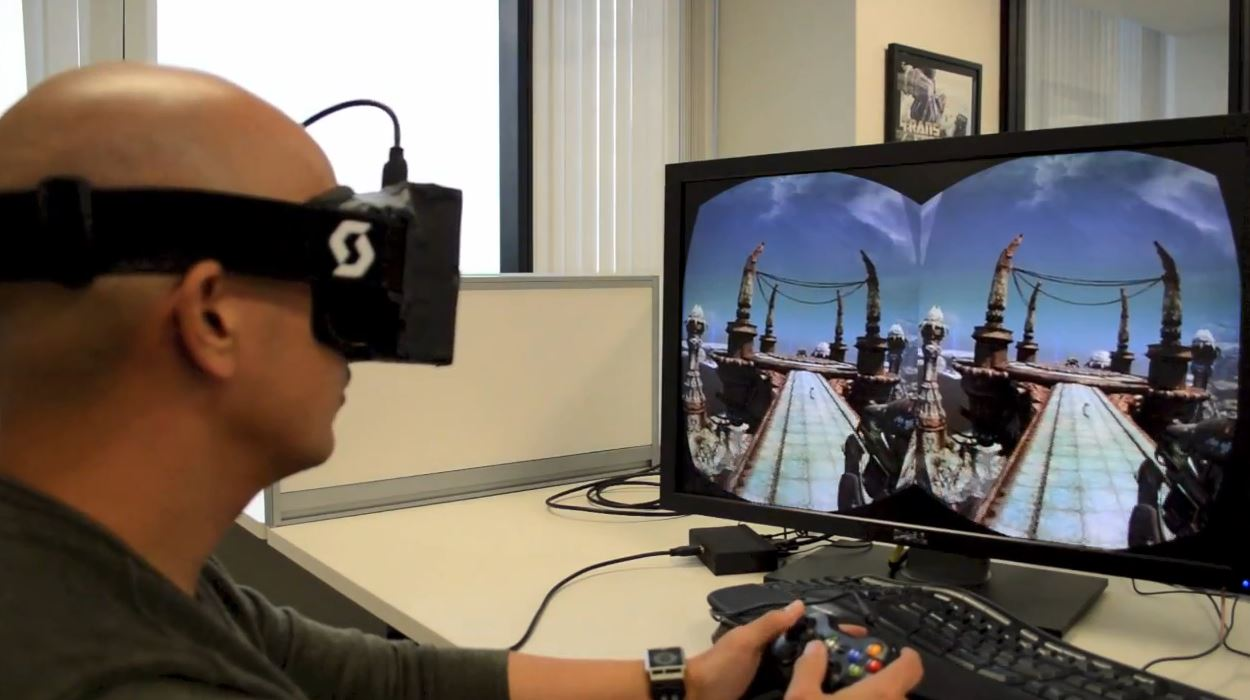
\includegraphics[scale=0.3]{2-Specifications/img-utilisateur/occulus.jpg}
\end{wrapfigure}
Lors de notre visite au centre de Kerpape nous avons fait essayer une démonstration de l'Occulus Rift à Willy Allègre et Jean-Paul Departe, qui ont été plutôt convaincus de l'intérêt du dispositif. Néanmoins, il s'agit d'une technologie onéreuse et dont le centre ne dispose pas actuellement.

\subsubsection{Salle immersive}
La salle immersive représente l'équipement de RV le plus complet dont nous puissions profiter et est donc une perspective de plate-forme très intéressante pour notre application.
\begin{wrapfigure}{l}{0mm}
	\centering
	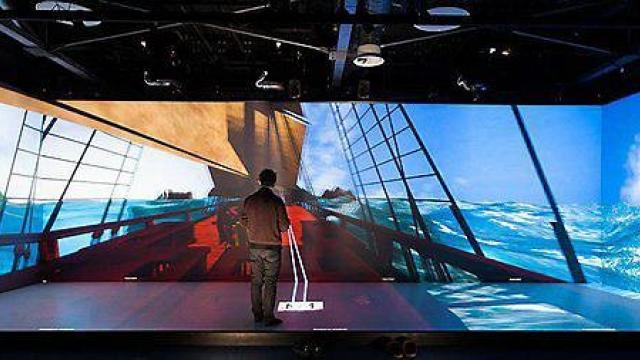
\includegraphics[scale=0.5]{2-Specifications/img-utilisateur/immersia.jpg}
\end{wrapfigure}
C'est l'option qui nous permettra les interactions les plus naturelles, car l'utilisateur se trouvera dans une projection à l'échelle 1:1 de l'appartement, équipé de lunettes 3D et de capteurs qui permettent de suivre la position des mains de l'utilisateur. \newline

Bien que Kerpape n'en dipose pas et n'ait pas la possibilité d'en utiliser une, l'implémentation du projet Avalon dans une salle immersive reste donc un objectif que nous souhaitons réaliser.

\pagebreak
\section{Architecture générale}
	\subsection{Briques logicielles}
		Notre projet peut être séparé en plusieurs briques logicielles ; celles-ci correspondent à une première ébauche de l'architecture globale du programme.
		\subsubsection{Moteur de rendu : Unity}
			La première brique est Unity; nous l'utiliserons ici pour sa composante moteur de jeu et environnement de développement, et non pour ses fonctionnalités de création d'objets 3d et ... 
		\subsubsection{Gestion des périphériques : MiddleVR}
			(DEJA FAIT en 2)Raison de son utilisation (multiples périphériques …)
		\subsubsection{Interactions avec les objets}
			Nous allons devoir développer un systême d'interractions entres les objets, pour qu'une action sur un objet ait un effet sur un autre objet.
		\subsubsection{Gestion des scénarios}
			Les scénarios demandés dans le cahier des charges devront être implémentés; il pourrait être appréciable que de nouveaux scénarios puissent facilement être ajoutés.
			De ce fait, nous avons besoin d'un système de gestion des scénarios qui devra par exemple donner l'ordre de différentes actions à réaliser par l'utilisateur, et d'éventuelles aides supplémentaires s'il devait réaliser une action autre que celle demandée.
		\subsubsection{Gestions des objets manipulables}
			Nous devrons aussi implémenter de quoi gérer les objets, pour pouvoir les retrouver et les gérer dans l'espace.
		\subsubsection{Menu}
			Un menu devra être disponible au lancement de l'application, ainsi qu'au cours de l'utilisation.
	\subsection{Liens entre les modules}

%MiddleVR <=> Unity
%Gestionnaire d’objets <=> Objets
%Gestionnaire scénarios <=> Gestionnaire d’objets
\pagebreak
\section{Conclusion}

Nous avons donc choisi une méthode fortement inspirée du cycle de production en V mais en la mêlant à des méthodes agiles pour pouvoir présenter le projet à nos clients régulièrement. Ainsi si chaque jalon du projet, représenté par un livrable à rendre, correspond à une étape de notre cycle en V, nous prévoyons en parallèle d'avancer le développement de l'application, en en présentant les itérations successives à Jean-Paul Departe et Willy Allègre. \newline

Ainsi, nos commanditaires peuvent valider notre avancée en quasi-temps réel. De plus, d'après l'audit réalisé sur Microsoft Project, nous disposons d'une planification correcte. Les différents livrables seront réalisés dans les temps et les estimations que nous avons faites tiennent compte des contre-temps que nous sommes susceptibles de rencontrer et devraient suffire à absorber les retards.

\end{document}
